\documentclass[border=8pt]{standalone}
\usepackage{tikz}
\usetikzlibrary{positioning}
\begin{document}
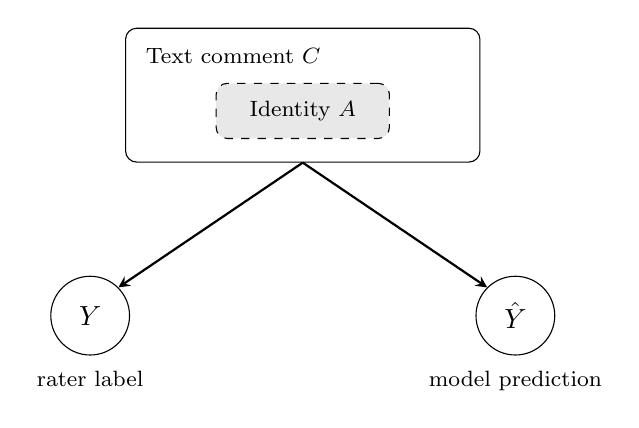
\begin{tikzpicture}[
  >=stealth,
  outnode/.style={draw, circle, minimum size=1cm}
]
  \node[draw, rounded corners, minimum width=4.5cm, minimum height=1.7cm] (C) at (0,0) {};
  \node[anchor=north west, font=\footnotesize] at ([xshift=4pt,yshift=-4pt]C.north west) {Text comment $C$};
  \node[draw, dashed, fill=gray!18, rounded corners, minimum width=2.2cm, minimum height=0.7cm, font=\footnotesize] (A) at (0,-0.2) {Identity $A$};
  \node[outnode](Y) at (-2.7,-2.8) {$Y$};
  \node[outnode](Yhat) at (2.7,-2.8) {$\hat Y$};
  \node[below=2pt of Y, font=\footnotesize] {rater label};
  \node[below=2pt of Yhat, font=\footnotesize] {model prediction};
  \draw[->, thick] (C.south) -- (Y.north east);
  \draw[->, thick] (C.south) -- (Yhat.north west);
\end{tikzpicture}
\end{document}
